\begin{figure}[h]
	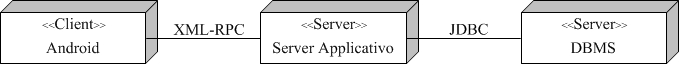
\includegraphics[width=\textwidth]{Immagini/Architecture_Envisoring}
	\caption{Architecture Envisioning}
	\label{fig:ArchitectureEnvisoring}
\end{figure}
\noindent
In figura ~\ref{fig:Deployment Diagram} e ~\ref{fig:ArchitectureEnvisoring} sono mostrati il Deployment Diagram e l'Architecture Envisioning del sistema progettato per lo sviluppo dell’applicazione di Book Crossing. Si può osservare che si tratta di un’architettura \textbf{\textit{Three Tiers}}:
\begin{enumerate}
	\item A sinistra si individua il client, ovvero il dispositivo Android con il quale è possibile interfacciarsi. Al suo interno quindi si può osservare la presenza di un componente relativo all’interfaccia grafica e uno relativo alla gestione delle richieste per invio e ricezione di dati con il server;
	\item Nella parte centrale individuiamo gli altri due layer dell’architettura: server EC2 e Database Relazionale RDS. il fatto di utilizzare Amazon Web Services consente di avere questi due elementi a bordo di un unico strato.
\end{enumerate}
\noindent
Per quanto riguarda la comunicazione tra i vari layer si sfruttano protocolli e librerie fornite sempre dall'ambiente Amazon Web Services. Nel caso della comunicazione tra smartphone e server EC2 si sfrutta Amazon SDK(nota con link), mentre per interfacciarsi con il Database RDS si sfrutta il connettore JDBC.